\documentclass[a4paper, 12pt, parskip=half-]{scrartcl}
\usepackage{tikz}
\usepackage{tkz-tab}
\usepackage{tkz-euclide}
\usepackage{xsim}
\usepackage{graphicx}
\usepackage{enumitem}
\setlist[enumerate]{label=\textbf{ \arabic*)}}
\usepackage{multicol}
\usepackage{amsmath}
\usepackage{tabularray}
\usepackage{mathtools}
\usepackage{cmbright}
\usepackage[french]{babel}
\usepackage[T1]{fontenc}
\usepackage{tasks}
\settasks{
    label-width=12pt
}
\usepackage{frenchmath}
\usepackage[export]{adjustbox}
\settasks{label=\textbf{\arabic*)}}
\usepackage[margin=1in]{geometry}
%\usepackage{showframe}

\begin{document}

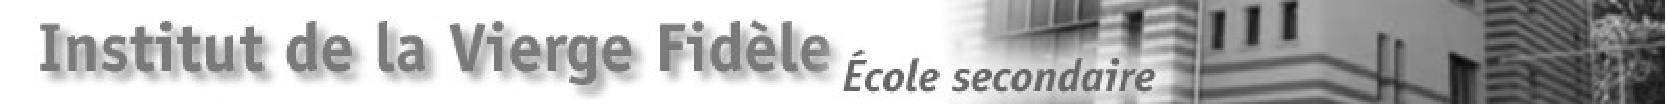
\includegraphics[width=\linewidth]{img/entete.pdf}\\
 {\scriptsize  30, rue de Linthout – 1030 Bruxelles}\\
    \begin{tblr}{hlines, vlines,
        colspec={XXX},
        cell{1}{1}={r=1, c=3}{c, font=\bfseries},
        cell{2}{1}={r=1, c=3}{c},
        cell{3}{1}={r=1, c=3}{c},
        cell{7}{1}={r=1, c=3}{l},
        hline{2,5,6}={white},
        vline{2,3}={white},
        }
        TRAVAIL DE REMISE A NIVEAU&& \\
        Mathématiques&& \\
        M. Baudoin - M. Tanghe \\
        Année: 2021-2022&Classe:&Numéro: \\
        &Nom:& \\
        Session : Août&Prénom:& \\
        Type de contrôle : écrit&& \\
    \end{tblr}           


Afin de te préparer au mieux ton contrôle écrit du 29 août, l'école te conseil de:
\begin{enumerate}
    \item Faire ou refaire les exercices de l'actimath dont les corrections se trouvent sur smartschool.\\
    Voici une liste non-exhaustive des exercices pouvant être fait:
    \begin{itemize}
        \item Chapitre 2 : activité 4.
        \item Chapitre 3 : activité 8.
        \item Chapitre 4 : activité 3 et 4.
        \item Chapitre 5 : activité 4 et 5.
        \item Chapitre 6 : analyse complète de fonction.
        \item Chapitre 7 : activité 4.
        \item Chapitre 8 : activité 8.
        \item Chapitre 9 : activité 2, 3 et 4.
        \item Chapitre 10 : activité 3, 4, 5 et 6.
        \item Chapitre 11 : activité 3, 5 et 8.
        \item Chapitre 12 : rien.
        \item Chapitre 13 : activité 5 ex 5.
        \item Chapitre 14 : activité 5 et 7.
    \end{itemize}
    \item Faire les exercices de drill ci-dessous dont les solutions arriverons début juillet.
    \item Si tu as besoin d'aide ou d'exercices supplémentaires, va voir les vidéos Youtube d'Yvan Monka ou va sur Khan academy afin de suivre les modules de troisième année (la théorie et des exercices y sont disponibles).
    \end{enumerate}
%%%%%%%%%%%%%%%% Exercise %%%%%%%%%%%%%%%%%%%%%
\newpage
\begin{exercise}
    Factorise les expressions suivantes:
    \begin{multicols}{2}
    \begin{enumerate}
        \item $6x^{3}+3x^{2}-9x+12$
        \item $3x^{4}-2x^{3}+5x^{2}$
        \item $7x^{4}-21x^{2}+14$
        \item $5xy^{2}+10x^{3}y$
        \item $81x^{3}-9y^{5}$
        \item $5xyz-10z^{2}$
        \item $8x^{3}+12x^{2}-20x$ 
        \item $6x^{2}+9x+4xy+6y$
        \item $10xy-10x+6y-6$
        \item $6x-8xz+15y-20z$
        \item $42xy-35x+16y-10$
        \item $-14xy-4x-35y-10$
        \item $-6jy-18j-3xy-9x$
        \item $10xyw-5w^{2}+6xy-3w$
        \item $-16x^{2}+36$
        \item $16x^{2}-16xy+4y^{2}$
        \item $9y^{2}-18xy+9x^{2}$
        \item $100-100y+25y^{2}$
        \item $25x^{2}-20x+4$
        \item $9y^{2}-12y+4$
        \item $4-4x+x^{2}$
        \item $64x^{2}+48xy+9y^{2}$
        \item $-4x^{4}+64x^{8}$
        \item $3x^{3}+4x^{2}-13x+6$
        \item $2x^{3}-5x^{2}-17x+20$
        \item $-3x^{3}-8x^{2}+7x+12$
        \item $-5x^{3}+22x^{2}-18x+40$
        \item $9x^{3}-3x^{2}+7x+1$
        \item $7x^{5}+7x^{4}+3x^{3}+3x^{2}+5x+5$
        \item $x^{2}-8x+15$
        \item $x^{2}+15x+56$
        \item $x^{2}+7x+12$
        \item $x^{2}+9x+14$
        \item $x^{2}+9x+18$
        \item $x^{2}+2x-15$
        \item $x^{2}-3x+54$
        \item $3x^{2}-6x+3$
        \item $-2x^{2}+18$
        \item $3x^{2}+12x+9$
        \item $-8x^{2}+12x-18$
        \item $3x^{2}-3x-6$
        \item $5x^{3}-70x+75$
        \item $9x^{3}+27x^{2}-x-3$
        \item $9x^{3}-36x^{2}+36x+9x-18$
        \item $27x^{4}-48x^{2}$
        \item $7x^{2}-21x-70$
        \item $24x^{3}-192x^{2}-40x+320$
        \item $-16x^{2}-16x+12$
        \item $2x^{3}+2x^{2}-2x-2$
        \item $21x^{2}-91x-70$
    \end{enumerate}
\end{multicols}
\end{exercise}
%%%%%%%%%%%%%%%%%% Solution %%%%%%%%%%%%%%%%%%%%%%
\begin{solution}
\begin{multicols}{2}
    \begin{enumerate}
        \item $3\left(2 x^{3} + x^{2} - 3 x + 4\right)$
        \item $x^{2}\left(3 x^{2} - 2 x + 5\right)$
        \item $7 \left(x - 1\right) \left(x + 1\right) \left(x^{2} - 2\right)$
        \item $5xy\left(2x^2+y\right)$
        \item $9 (9 x^3 - y^5)$
        \item $5z(xy-2z)$
        \item $4x(2x+5)(x-1)$
        \item $(2x+3)(3x+2y)$
        \item $2(y-1)(5x+3)$
        \item $6x-8xz+15y-20z$
        \item $42xy - 35x + 16y - 10$
        \item $-(2 x + 5)(7 y + 2)$
        \item $-3(y+3)(2j+x)$
        \item $(2xy-w)(5w+3)$
        \item $4(3-2x)(3+2x)$
        \item $4(2x-y)^2$
        \item $9(y-x)^2$
        \item $25(2-y)^2$
        \item $(5x-2)^2$
        \item $(3y-2)^2$
        \item $(2-x)^2$
        \item $(8x+3y)^2$
        \item $4x^4(2x-1)(2x+1)(4x^2+1)$
        \item $(x-1)(x+3)(3x-2)$
        \item $(x-1)(2x+5)(x-4)$ 
        \item $-(x+1)(x+3)(3x-4)$
        \item $-(x-4)(5x^2-2x+10)$
        \item $9x^3-3x^2+7x+1$
        \item $\left(7x^4 + 3x^2 + 5\right)(x+1)$
        \item $(x-3)(x-5)$
        \item $(x+8)(x+7)$
        \item $(x+4)(x+3)$
        \item $(x+7)(x+2)$
        \item $(x+6)(x+3)$
        \item $(x+5)(x-3)$
        \item $x^2 - 3x + 54$
        \item $3(x-1)^2$ 
        \item $-2(x-3)(x+3)$
        \item $3(x+3)(x+1)$
        \item $-2\left(4x^2 - 6x + 9\right)$
        \item $3(x+1)(x-2)$
        \item $5(x-3)(x^2+3x-5)$
        \item $(x+3)(3x-1)(3x+1)$
        \item $9(x-1)^2(x-2)$
        \item $3x^2(3x-4)(3x+4)$
        \item $7(x+2)(x-5)$
        \item $8(x-8)\left(3x^2 - 5\right)$
        \item $-4(2x+3)(2x-1)$
        \item $2(x+1)^2(x-1)$
        \item $7(3x+2)(x-5)$               
    \end{enumerate}
\end{multicols}
\end{solution}
%%%%%%%%%%%%%%%%% Exercise %%%%%%%%%%%%%%%%%%%%%%%
\newpage
\begin{exercise}
    Détermine les valeurs de $x$.
    \begin{tasks}[after-item-skip=\fill](2)
        \task \input{tikz/Triangle_001.tikz}
        \task \begin{tikzpicture}[rotate=15, baseline=(current bounding box.north)]
    \tkzDefPoint(0,0){A}
    \tkzDefPoint(0,-4){B}
    \tkzDefPoint(3,-4){C}
    \tkzDrawPolygon(A,B,C)
    \tkzLabelPoints[left](A)
    \tkzLabelPoints[below right](C)
    \tkzLabelPoints[below left](B)
    \tkzLabelSegment(A,C){$15$}
    \tkzLabelSegment[left](A,B){$9$} 
    \tkzLabelSegment[below](B,C){$x$}
    \tkzDrawPoints(A,B,C)
    \tkzMarkRightAngle[size=.5](A,B,C)
\end{tikzpicture}
        \task \begin{tikzpicture}[rotate=-20, baseline=(current bounding box.north)]
    \tkzDefPoint(0,0){A}
    \tkzDefPoint(0,-4){B}
    \tkzDefPoint(3,-4){C}
    \tkzDrawPolygon(A,B,C)
    \tkzLabelPoints[above](A)
    \tkzLabelPoints[below right](C)
    \tkzLabelPoints[below left](B)
    \tkzLabelSegment(A,C){$x$}
    \tkzLabelSegment[left](A,B){$8$} 
    \tkzLabelSegment[below](B,C){$17$}
    \tkzDrawPoints(A,B,C)
    \tkzMarkRightAngle[size=.5](A,B,C)
\end{tikzpicture}
        \task \begin{tikzpicture}[rotate=135, baseline=(current bounding box.north)]
    \tkzDefPoint(0,0){A}
    \tkzDefPoint(0,-4){B}
    \tkzDefPoint(3,-4){C}
    \tkzDrawPolygon(A,B,C)
    \tkzLabelPoints[below left](A)
    \tkzLabelPoints[above](C)
    \tkzLabelPoints[right](B)
    \tkzLabelSegment(A,C){$x$}
    \tkzLabelSegment[below right](A,B){$81$} 
    \tkzLabelSegment[above right](B,C){$49$}
    \tkzDrawPoints(A,B,C)
    \tkzMarkRightAngle[size=.5](A,B,C)
\end{tikzpicture}
        \task \begin{tikzpicture}[rotate=-79, baseline=(current bounding box.north)]
    \tkzDefPoint(0,0){A}
    \tkzDefPoint(0,-4){B}
    \tkzDefPoint(3,-4){C}
    \tkzDrawPolygon(A,B,C)
    \tkzLabelPoints[right](A)
    \tkzLabelPoints[below](C)
    \tkzLabelPoints[left](B)
    \tkzLabelSegment(A,C){$x$}
    \tkzLabelSegment[above](A,B){$\sqrt{40}$} 
    \tkzLabelSegment[left](B,C){$\sqrt{24}$}
    \tkzDrawPoints(A,B,C)
    \tkzMarkRightAngle[size=.5](A,B,C)
\end{tikzpicture}
        \task \begin{tikzpicture}[rotate=-189, baseline=(current bounding box.north)]
    \tkzDefPoint(0,0){A}
    \tkzDefPoint(0,-4){B}
    \tkzDefPoint(3,-4){C}
    \tkzDrawPolygon(A,B,C)
    \tkzLabelPoints[below](A)
    \tkzLabelPoints[left](C)
    \tkzLabelPoints[right](B)
    \tkzLabelSegment(A,C){$14$}
    \tkzLabelSegment[right](A,B){$x$} 
    \tkzLabelSegment[above](B,C){$\sqrt{100}$}
    \tkzDrawPoints(A,B,C)
    \tkzMarkRightAngle[size=.5](A,B,C)
\end{tikzpicture}
    \end{tasks}
\end{exercise}
%%%%%%%%%%%%%%%%% Solution %%%%%%%%%%%%%%%%%%%%%%%
\begin{solution}
    \begin{enumerate}
        \item Impossible.
        \item $12$
        \item $\sqrt{353}$
        \item $\sqrt{8962}$
        \item $8$
        \item $4\sqrt{6}$
    \end{enumerate}
\end{solution}
%%%%%%%%%%%%%%%%% Exercise %%%%%%%%%%%%%%%%%%%%%%%
\newpage
\begin{exercise}
    Détermine les conditions d'existences puis simplifie en factorisant.
    \begin{multicols}{2}
        \begin{enumerate}
            \item $\dfrac{2x^{2}-7x+6}{x^{2}-2x}\cdot\dfrac{14x+21}{x^{2}-2x}$
            \item $\dfrac{3x-15}{4x-12}\cdot\dfrac{x-5}{8x-24}$
            \item $\dfrac{16x^{2}+48x+36}{16x^{2}-36}\cdot\dfrac{2x^{2}+2x-3x-3}{5}$
            \item $\dfrac{-8x+36}{x^{2}+2x+1}\cdot\dfrac{x^{2}-1}{-4x+18}$
        \end{enumerate}        
    \end{multicols}
\end{exercise}
%%%%%%%%%%%%%%%%% Solution %%%%%%%%%%%%%%%%%%%%%%%
\begin{solution}
    \begin{multicols}{2}
        \begin{enumerate}
            \item $\dfrac{28x^2 - 63}{x^3-2x^2}$ \quad si $x \ne 0$ et $x \ne 2$
            \item $\dfrac{3x^2 - 30x + 75}{32x^2 - 192x + 288}$ \quad si $x \ne 3$
            \item $\dfrac{2x^2 + 5x + 3}{5}$ \quad si $x \ne \pm \dfrac{3}{2}$
            \item $\dfrac{2x-2}{x+1}$ \quad si $x \ne -1$ et $ x \ne \dfrac{9}{2}$   
        \end{enumerate}
    \end{multicols}
\end{solution}
%%%%%%%%%%%%%%%% Exercise %%%%%%%%%%%%%%%%%%%%%%
\begin{exercise}
  Pour chacune des fonctions ci-dessous, détermine:
  \begin{multicols}{3}
    \begin{itemize}
        \item Le domaine
        \item L'ensemble images
        \item Les racines
        \item L'ordonnée à l'origine
        \item Le tableau de signes
        \item Le tableau de variation
      \end{itemize}
  \end{multicols}

  \begin{tasks}(2)
        \task 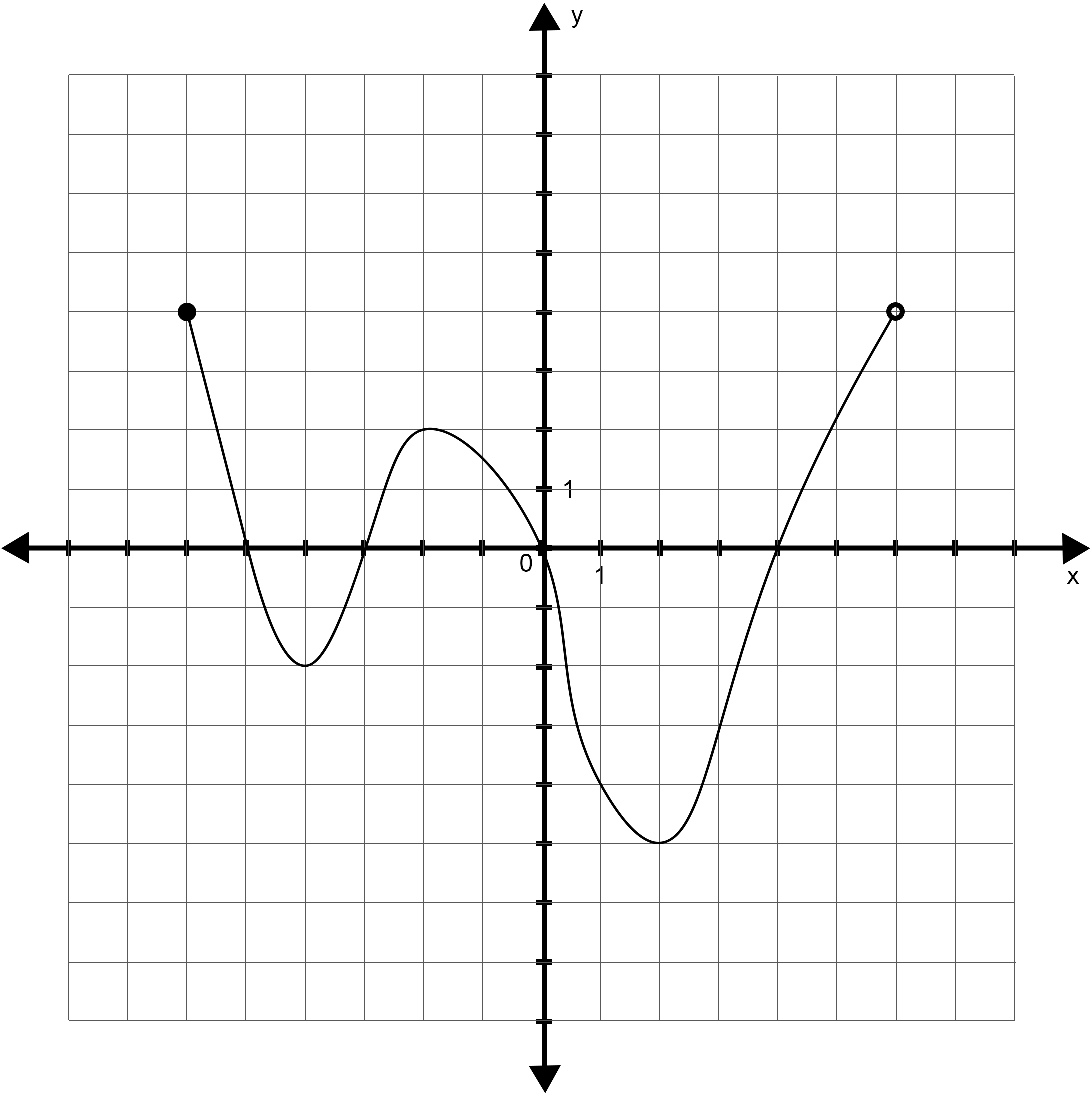
\includegraphics[valign=t, width=\linewidth]{img/EtudeFct_01.pdf}
        \task 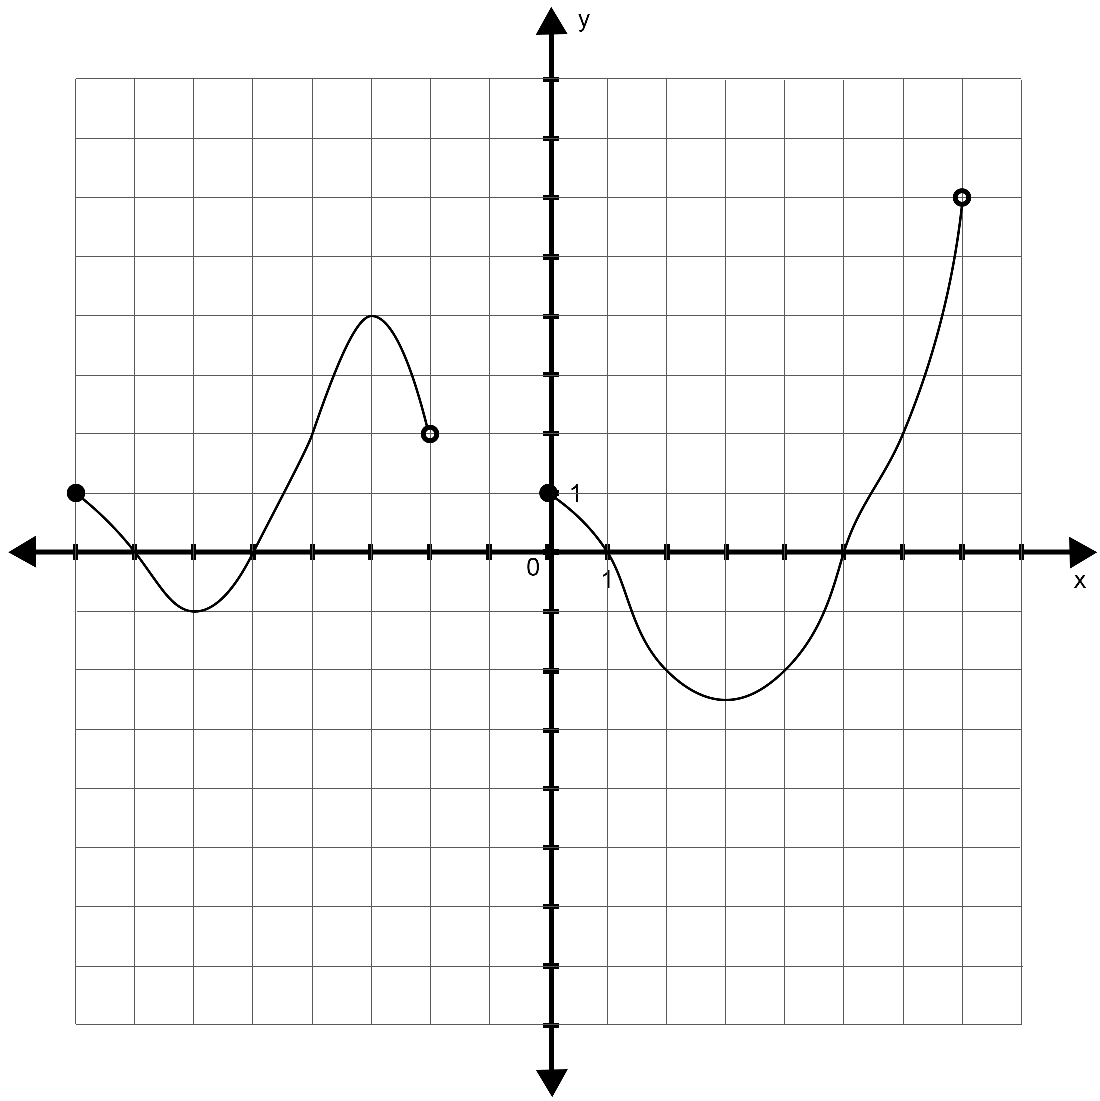
\includegraphics[valign=t, width=\linewidth]{img/EtudeFct_02.pdf}
        \task 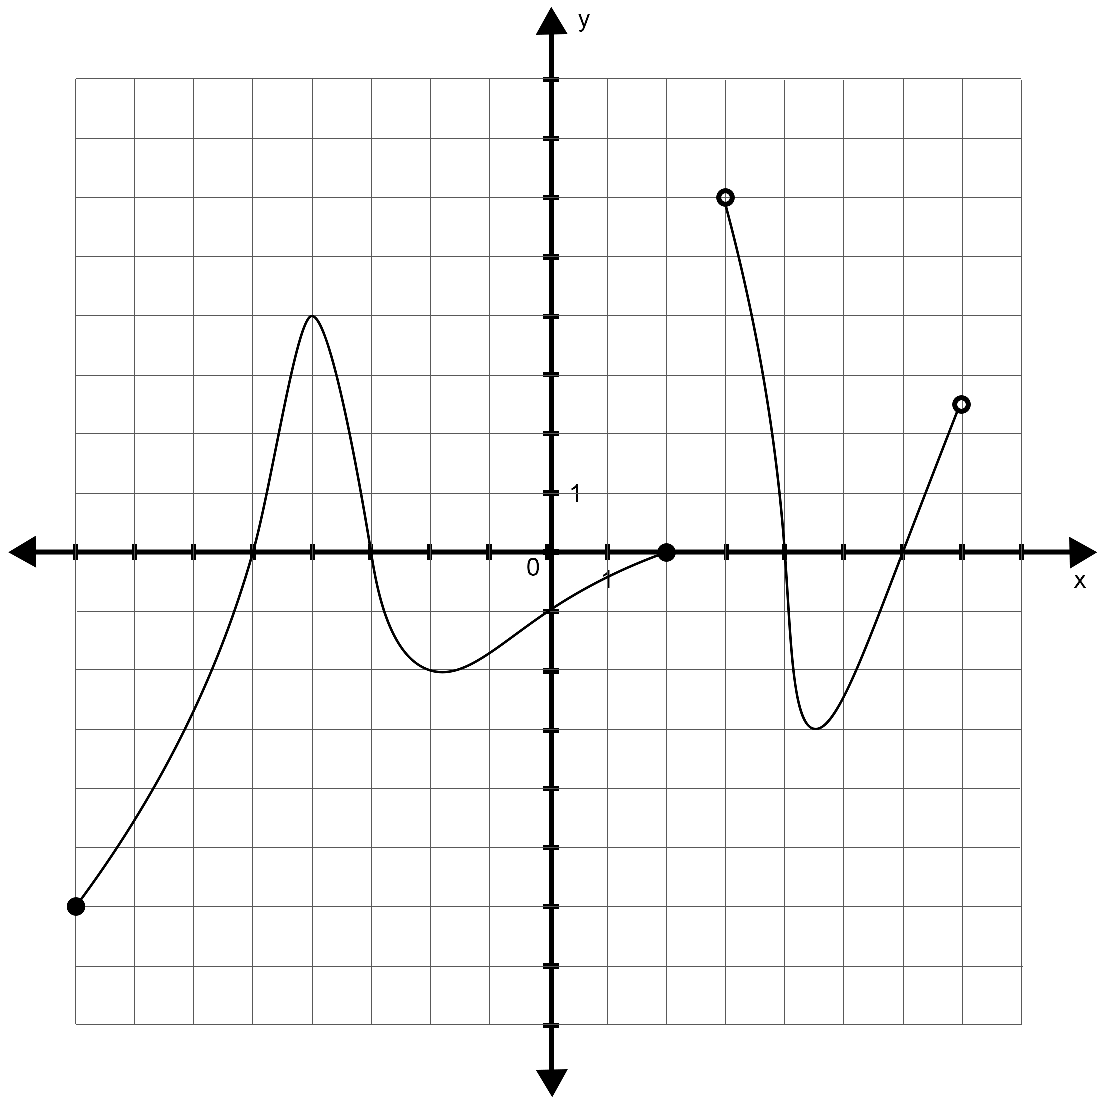
\includegraphics[valign=t, width=\linewidth]{img/EtudeFct_03.pdf}
      \end{tasks}

\end{exercise}
%%%%%%%%%%%%%%%% Solution %%%%%%%%%%%%%%%%%%%%%%
\begin{solution}
    \begin{enumerate}
        \item 
        \begin{itemize}
            \item $dom~f = [-6;6[$ 
            \item $im~f = [-5;4]$
            \item Racine(s) : $\lbrace -5; -3; 0; 4\rbrace$
            \item Ordonnée à l'origine : $0$
            \item Tableau de signes\medbreak
            \begin{tikzpicture}
                \tkzTabInit[espcl=1.5]%
                {$x$/1, $f(x)$/1}%
                {$-6$, $-5$, $-3$, $0$, $4$, $6$}
                \tkzTabLine{+, +, z, -, z, +, z, - ,z,+,d}
            \end{tikzpicture}
            \item Tableau de variations\medbreak
            \begin{tikzpicture}
                \tkzTabInit[espcl=1.5]%
                {$x$/1, $f(x)$/2}%
                {$-6$, $-4$, $-2$, $2$, $6$}
                \tkzTabVar{+/$4$, -/$-2$,+/$2$,-/$-5$,+D/}
            \end{tikzpicture}
        \end{itemize}
        \item 
        \begin{itemize}
            \item $dom~f = [-8;-2[ ~\cup~ [0;7[$ 
            \item $im~f = [-2,5; 6[$
            \item Racine(s) : $\lbrace -7; -5; 1; 5 \rbrace$
            \item Ordonnée à l'origine : $1$
            \item Tableau de signes\medbreak
            \begin{tikzpicture}
                \tkzTabInit[espcl=1.5]%
                {$x$/1, $f(x)$/1}%
                {$-8$ , $-7$, $-5$, $-2$, $0$,  $1$, $5$, $7$}%
                \tkzTabLine{+, +, z, -, z, +, d, h, +, +, z, -, z , + , d}
            \end{tikzpicture}
            \item Tableau de variations\medbreak
            \begin{tikzpicture}
                \tkzTabInit[espcl=1.5]%
                {$x$/1, $f(x)$/2}%
                {$-8$, $-6$, $-3$, $-2$, $0$, $3$, $7$}
                \tkzTabVar{+/$1$, -/$-1$,+/$-4$, -DH/, +/$1$, -/{$-2,5$}, +D/}
            \end{tikzpicture}
        \end{itemize}
        \item
        \begin{itemize}
            \item $dom~f =[-8,2]~\cup~]3;7[$ 
            \item $im~f = [-6;6[$
            \item Racine(s) : $\lbrace -5; -3; 2; 4; 6 \rbrace$
            \item Ordonnée à l'origine : $-1$
            \item Tableau de signes\medbreak
            \begin{tikzpicture}
                \tkzTabInit[espcl=1.5]%
                {$x$/1, $f(x)$/1}%
                {$-8$, $-5$, $-3$, $2$, $3$, $4$, $6$, $7$}%
                \tkzTabLine{-, -, z, +, z, - , z, h, d, +, z, -, z, +, d}
            \end{tikzpicture}
            \item Tableau de variations\medbreak
            \begin{tikzpicture}
                \tkzTabInit[espcl=1.5]%
                {$x$/1, $f(x)$/2}%
                {$-8$, $-4$, $-2$, $2$, $3$, {$3,5$}, $7$}
                \tkzTabVar{-/$-6$, +/$4$, -/$-2$, +H/$0$, D+/, -/$-3$, +D/}
            \end{tikzpicture}
        \end{itemize}
    \end{enumerate}
\end{solution}
\newpage
\printsolutions
\end{document}